\chapter{Valutazione dei risultati}\label{ch:evaluation}

  \section{Considerazioni sul contributo}
    Il problema delineato nei~\Cref{ch:requirements,ch:project} prevedeva la realizzazione di un sistema per l'esecuzione di codice Protelis attraverso una piattaforma web, appoggiandosi ad una rete di dispositivi simulata.
    I requisiti funzionali sono stati tutti soddisfatti:
    la Single-Page Application realizzata permette di visualizzare e modificare il codice Protelis all'interno del campo editor e fornisce una rappresentazione dei risultati attraverso un canvas che disegna l'output.
    L'utente non deve configurare impostazioni complesse:
    l'unica configurazione messa a disposizione, oltre ovviamente al codice da eseguire, è la selezione del server di backend.
    Anche il server soddisfa i propri requisiti funzionali:
    l'esecuzione del codice è delegato a singole istanze del simulatore Alchemist, le quali generano ciascuna una rete virtuale, in modo da poter servire ciascuno degli utenti del sistema in contemporanea.

    Il client soddisfa appieno anche i requisiti non funzionali:
    l'esperienza utente è immediata, con un'interfaccia orizzontale responsiva strutturata su una singola pagina.
    La configurazione dei polyfill permette il supporto a tutti i browser con percentuali di utilizzo superiori allo \SI{0.2}{\percent} e che non abbiano terminato il supporto ufficiale da più di 24 mesi;
    lo strumento \texttt{browserlist} stima una copertura del \SI{91.67}{\percent} delle piattaforme correntemente utilizzate.
    Anche il protocollo impiegato per la comunicazione con il server, SockJS, risulta compatibile con la maggior parte delle piattaforme in uso, utilizzando però soluzioni di trasporto meno efficienti su browser più datati.
    Infine, il server soddisfa il requisito di scalabilità, garantito principalmente dalle possibilità fornite dal framework Vert.x.

    Il sistema inoltre è stato progettato con diverse possibilità di espansione in mente, principalmente per quanto riguarda il supporto ad altri linguaggi (come ScaFi) e ad altri motori di esecuzione.
    Si tratterà meglio questo aspetto nel~\Cref{ch:considerations}.

    L'unica problematica individuata riguarda l'efficienza:
    la costruzione di una nuova simulazione Alchemist per ogni utente che richieda un'esecuzione comporta tempi di costruzione e impiego di memoria non banali (soprattutto su piattaforme cloud gratuite come Heroku \emph{Free}).
    Questo problema è strettamente legato alla necessità dei linguaggi aggregati di eseguire su una rete e può essere solamente aggirato tramite meccanismi di caching o scalando il sistema aumentando le risorse a disposizione.

  \section{Valutazione dell'interfaccia}
    Per quanto riguarda la valutazione della qualità dell'interfaccia web realizzata, è stata presa in considerazione principalmente l'esperienza finale dal punto di vista dell'utente web.
    Per avere una misura quantitativa di quanto l'applicazione web si presenti adeguata, si è deciso di utilizzare lo strumento Lighthouse messo a disposizione da Google.

    \emph{Lighthouse} è uno strumento automatizzato open-source, fornito inizialmente con la suite di strumenti \emph{Chrome DevTools}, che permette l'\emph{auditing} di pagine web secondo gli standard premiati dal motore di ricerca di Google.
    Esso verifica le prestazioni di caricamento e navigazione, l'accessibilità, l'ottimizzazione per i motori di ricerca, e in generale le buone pratiche di programmazione.
    Supporta inoltre controlli aggiuntivi per le PWA (\emph{\emph{P}rogressive \emph{W}eb \emph{A}pp}) se abilitati.

    \begin{figure}[htbp]
      \centering
      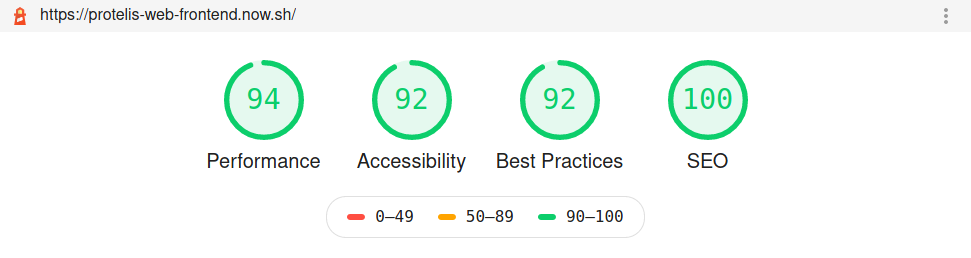
\includegraphics[width=\textwidth]{res/tests/Screenshot_2020-03-04 Lighthouse Report Viewer.png}% ChkTeX 8
      \caption{Punteggio ottenuto con Google Lighthouse}%
      \label{fig:lighthouse}
    \end{figure}

    Come è possibile vedere in~\Cref{fig:lighthouse}, un'analisi dell'applicazione web realizzata attraverso il plugin ufficiale per FireFox ha ottenuto un buon punteggio generale.
    Di seguito verranno analizzati i singoli valori separatamente.

    \subsection{Performance}
      Lighthouse ad ogni analisi assegna un punteggio denominato \emph{performance} basato su diverse metriche in relazione ai diversi stadi caricamento della pagina;
      i valori grezzi ottenuti per ciascuna metrica vengono mappati su una distribuzione log-normale derivata dalle metriche prestazionali ricavate da HTTPArchive\footnote{\url{https://httparchive.org/}}.
      0 è il minor valore possibile e generalmente indica un errore interno a Lighthouse, mentre 100 è il valore migliore, che posiziona la pagina analizzata nel 98-esimo percentile dei siti più performanti.

      Secondo lo strumento, le performance %, sulle quali si ha avuto maggiore controllo durante l'implementazione,
      del frontend di WebProtelis sono buone, con tempi di primo disegno inferiori al secondo e un ritardo prima di avere possibilità di interazione intorno a \SI{1.6}{\second}.
      A pesare un poco sul punteggio vi è l'assenza di gestione della cache delle richieste, funzionalità non ritenuta importante in questo progetto.

    \subsection{Accessibilità e Best Practices}

    Il punteggio denominato \emph{accessibility} è dato da una media ponderata dei numerosi audit di accessibilità effettuati;
    a differenza di quanto avveniva per le performance, ciascun audit non ha valori parziali, bensì solo 0 o 100.
    Anche il punteggio di \emph{best practices} è composto da diverse caratteristiche, delle quali viene ricavata una media non pesata.

    I punteggi ottenuti da questo progetto sono strettamente legati dalle librerie impiegate, sia in positivo che in negativo:
    il valore elevato deriva da ottimizzazioni della libreria stessa sui componenti che fornisce, cercando di aderire quanto possibile agli standard più moderni;
    le criticità che non portano al \SI{100}{\percent} sono legate a limiti difficilmente aggirabili se non configurazioni complesse e fuori tema rispetto all'obiettivo di questa tesi.

    \subsection{SEO}

    Infine, con \emph{SEO} si intende \emph{\emph{S}earch \emph{E}ngine \emph{O}ptimization}, ovvero quanto la pagina web è ottimizzata per la ricerca tramite motori come Google.
    Il punteggio è determinato dalla presenza dei corretti tag nel documento, che permettono alla pagina di essere analizzata e descritta in modo accurato.
    Nel caso di questo progetto, ottimizzando manualmente la configurazione base generata da React seguendo le specifiche documentate da Google, si è riuscito ad ottenere il massimo punteggio, che dovrebbe garantire un buon ranking nelle ricerche.

    % \section{Qualità del codice e unit testing}
    %   Durante lo sviluppo, si è cercato di prestare particolare attenzione alla qualità del codice prodotto.

    %   Si è ritenuto fondamentale, innanzitutto, per favorire la consistenza dello stile, che il codice fosse conforme a uno stile di programmazione riconosciuto.
    %   Come detto nella~\Cref{subec:quality}, sono stati utilizzati diversi \emph{linter} (ESLint e ktlint)
    %   per imporre lo stile Airbnb per TypeScript e lo stile ufficiale per Kotlin in tutta la codebase.
    %   Questo ha permesso di evitare bug comuni riconoscibili attraverso analisi statica
    %   e potenzialmente permette di rendere il codice, che è pubblico e open-source, maggiormente comprensibile per chi vorrà estenderlo in futuro.

    %   Inoltre, per garantire il corretto funzionamento delle componenti più cruciali, sono stati creati degli specifici unit test in grado di coprire il codice per quanto possibile.
    %   L'esecuzione dei test viene effettuata automaticamente da Travis CI su diverse piattaforma ad ogni operazione di push.

    %   Per quanto riguarda il backend è stato utilizzato JUnit 5 con l'ausilio delle estensioni di Vert.x.
    %   I report sulla copertura vengono raccolti tramite JaCoCo.

    %   \unsure[inline]{Quali dettagli dovrei fornire dei test del backend?}

    %   Anche il frontend è stato testato tramite unit testing.
    %   In particolare, si è utilizzato la suite Jest per l'esecuzione dei test e la raccolta dei dati di copertura.

    %   \unsure[inline]{Quali dettagli dovrei fornire dei test del frontend?}

    % \section{Performance}
    %   % TODO
    %   \unsure[inline]{Come valuto i risultati? Misure di Performance?}
